\documentclass[a4paper,12pt]{article}
\usepackage[utf8]{inputenc}
\usepackage[margin=0.6in]{geometry}
\usepackage{amsmath, amssymb, dsfont}
\usepackage[font=footnotesize]{caption}
\usepackage{braket}
\usepackage{lscape}
\usepackage{rotating}
\usepackage{hyperref}
\usepackage{xcolor}
\usepackage{subcaption}
\usepackage{graphicx}
\hypersetup{
    colorlinks,
    linkcolor={blue!70!black},
    citecolor={blue!70!black},
    urlcolor={blue!70!black}
}

\newcommand\todo[1]{\textcolor{red}{#1}}
\newcommand{\olsi}[1]{\,\overline{\!{#1}}} % overline short italic

%opening
\title{A primer on quantum RAM}
\author{Olivia Di Matteo}

\begin{document}

\maketitle

\abstract{\textcolor{red}{\textbf{This document is a work in progress} and is being continuously edited.}}
\setcounter{tocdepth}{4}
\setcounter{secnumdepth}{4}
\tableofcontents

\section{FAQ}

Quantum RAM (qRAM) has gained some notoriety in the past few years, and attitudes toward it depend quite heavily on the circles you run in. 
The goal of this set of notes is to provide a general overview of the subject, as well as discuss some very specific implementations. 
It is meant to be a companion to the Q\# qRAM libraries we are writing \cite{OurLibrary}, but can also serve as a standalone reference.


In my experience, explaining qRAM to someone boils down to answering a handful of key questions. 
I'll provide some potentially unsatisfactory answers up front, but go into far more detail in the next few sections\footnote{Those details may not be satisfactory either.}.

\begin{enumerate} 
 \item \textbf{Do I need a qRAM?}
  \emph{Sometimes}. You'll need a qRAM, or some more general means of \emph{quantum state preparation} in quantum machine learning (QML) algorithms that require you to load in classical data, or query an oracle that returns classical data. 
  I've heard a number of stories of people working on QML being actively discouraged from doing so because ``QML won't work without a qRAM''. 
  That's just not true, because \emph{many QML algorithms do not need a qRAM}.
  Now, whether or not they yield any quantum advantage is a separate question, and won't be discussed here. 
  The key point I want to make is that \emph{some} QML algorithms need a qRAM, and they will potentially run into trouble as per the next question.
 \item \textbf{Can we design an efficient qRAM?} \emph{Maybe.} 
 In this primer we'll take a look at proposals that will in principle run in polynomial depth, and others that scale far worse. 
 There are some very interesting qubit-time tradeoffs one can explore, in particular if the data being stored has some sort of underlying structure. 
 Regardless, even if we can design an efficient circuit, we'd also like something that is efficient in a fault-tolerant setting, and this is potentially very expensive.
 \item \textbf{Can I build one?} \emph{Maybe.} No one has actually done so, but there are a handful of hardware proposals that will be discussed in more detail in \autoref{sec:hardware}. 
\end{enumerate}

%%%%%%%%%%%%%%%%%%%%%%%%%%%%%%%%%%%%%%%%%%%%%%%%%%%%%%%%%%%%%%%%%%%%%%%%%%%%%%%%%%
%%%%%%%%%%%%%%%%%%%%%%%%%%%%%%%%%%%%%%%%%%%%%%%%%%%%%%%%%%%%%%%%%%%%%%%%%%%%%%%%%%
%%%%%%%%%%%%%%%%%%%%%%%%%%%%%%%%%%%%%%%%%%%%%%%%%%%%%%%%%%%%%%%%%%%%%%%%%%%%%%%%%%
%%%%%%%%%%%%%%%%%%%%%%%%%%%%%%%%%%%%%%%%%%%%%%%%%%%%%%%%%%%%%%%%%%%%%%%%%%%%%%%%%%
%%%%%%%%%%%%%%%%%%%%%%%%%%%%%%%%%%%%%%%%%%%%%%%%%%%%%%%%%%%%%%%%%%%%%%%%%%%%%%%%%%

\section{Introduction}

\subsection{Classical memory}

Random access memory (RAM) is an integral part of modern-day computers.
It's what stores the active state of a computation, or data that you might actively be processing. 
The more RAM you have, the more applications you can have open simultaneously.
At the time of writing, the average laptop computer comes with about 8 or 16 GB. 
RAM is plentiful, and it is also reasonably cheap - you can outfit a desktop computer with 16 GB RAM for about 100\$ CAD. 
Considering that some of the earliest personal computers had only 4 KB of RAM, the technology has come a long way, and is continuously improving.

\begin{figure}[ht]
 \centering
  \captionsetup{width=.89\linewidth}
 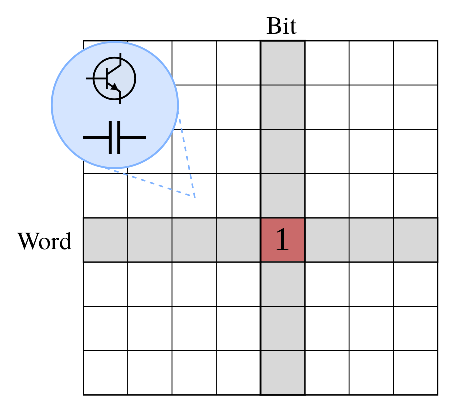
\includegraphics[scale=0.8]{images/memory-models}
 \caption{Cartoon depiction of RAM as a 2-dimensional array of transistor/capacitor pairs.
 Rows are called \emph{wordlines}, and columns are called \emph{bitlines}.
 Control electronics can write to and read contents of arbitrary cells, hence the term `random access'.}
 \label{fig:memory-models}
\end{figure}

A simplified model of RAM is shown in \autoref{fig:memory-models}. 
It's depicted as a 2-dimensional array of memory cells where a capacitor and transistor live together. 
A capacitor can either hold a charge, or not hold a charge - this can be used to represent a 1 or a 0 respectively. 
The transistors are essentially control electronics. 
By sending current through particular rows (wordlines) and columns (bitlines) of the grid, you can read or write to arbitrary memory cells (hence `random access' memory).


Unfortunately, charge leaks out of the capacitors over time.
To preserve the integrity of the data, a \emph{memory controller} continuously performs a refresh operation.
It scans across all memory cells, reads their contents, and then immediatley writes them back.
The frequency at which this is done is called the refresh rate.
In addition to the charge degrading over time, the capacitors hold charge only when powered.
Thus when you turn off your computer, everything stored in your RAM disappears.

The cousin of RAM is ROM, or read-only memory.
In its most basic form\footnote{In fact there are a variety of different ROMs, many of which are in fact reprogrammable. See \url{
https://studyelectrical.com/2017/06/different-types-of-rom-prom-eprom.html} for a brief and accessible overview of the different types.} data is written to a ROM only once, and subsequent interaction involves only reading said data.
Essentially, ROM is like a look-up table.
Unlike RAM, the data stored in ROM does persist when its powered off. 
ROM therefore has applications in things like special-purpose appliances, old video game cartridges, and even parts of modern processors.
\todo{Give some specific examples - CDs, flash memory, etc.}

\subsection{Encoding classical data on a quantum computer}
\label{sec:encoding}

Given the importance of ROM and RAM for classical hardware, it's not unreasonable to assume that quantum computers will require something conceptually similar, a qRAM or qROM.
In this work (and in the Q\# library), we consider the problem of how to load up and store \emph{classical} data on a quantum computer.
One of the key applications is of course quantum machine learning.
However many other quantum algorithms rely on things like \emph{quantum state preparation} based on classical data, or look up tables.
\todo{Include some examples.}

A number of different methods can be used to load classical data onto a quantum machine.
Consider an arbitrary $n$-qubit quantum state
\begin{equation}
 \ket{\psi} = \sum_{\mathbf{x} \in \{0, 1\}^n} \alpha_{\mathbf{x}} \ket{\mathbf{x}}, \quad \alpha_{\mathbf{x}} \in \mathds{C}.
\end{equation}
There are two aspects in which we can consider encoding the classical information:
\begin{enumerate}
 \item Incorporate into the amplitudes $\alpha_{\mathbf{x}}$
 \item Incorporate into the qubit basis states $\ket{\mathbf{x}}$
\end{enumerate}
The subsections below elaborate on different examples of each, however only one of these is what's traditionally defined as qRAM.
This list is not exhaustive, and for a more in-depth overview see Chapter 5 of the excellent quantum machine learning textbook \cite{Schuld2018}.

\subsubsection{Quantum RAM / ROM}
Suppose we have some classical data represented as $m$-bit strings, $\mathbf{b} \in \{0, 1\}^m$. 
For simplicity, assume there are $N = 2^n$ such strings.
We can store these bit strings in a memory by setting up a set of $N$ memory cells addressed by $n$ bits, such that the address $\mathbf{x} \in \{0, 1\}^n$ contains the $m$-bit string $\mathbf{b}_{\mathbf{x}}$.
For example, let $n = 3$ and $m = 4$.
A memory would look something like this:
\begin{equation}
 \begin{tabular}{c|c}
  \hbox{Address (}$\mathbf{x}$) & \hbox{Contents (}$\mathbf{b}_{\mathbf{x}})$ \\ \hline
  000 & 0110 \\
  001 & 1000 \\
  010 & 1011 \\ 
  $\vdots$ & $\vdots$
  \end{tabular}
  \label{eq:qram_table}
\end{equation}
In the general case where $N$ is not a power of 2, $n = \lceil \log_2 N \rceil$ bits would be required to express the addresses, and the contents of a number of the cells would simply be $m$ 0s.

A qRAM (or similarly a qROM) is a unitary operation that \emph{queries} the contents of these memory cells in superposition. 
The operation works on two quantum registers (sets of qubits): the first encodes the addresses, and the second is there to hold the memory contents after the query.
We call these the address register and output register respectively.
Expressed mathematically, a qRAM/qROM performs the operation
\begin{equation}
 \sum_{\mathbf{x}} \ket{\mathbf{x}} \ket{0} \rightarrow \sum_{\mathbf{x}} \ket{\mathbf{x}} \ket{\mathbf{b}_{\mathbf{x}}},
\end{equation}
where for simplicity we have ignored the amplitudes.
Using \autoref{eq:qram_table} as example data, the qRAM effects the transformation
\begin{equation}
 \left(\ket{000} + \ket{001} + \ket{010} + \cdots \right) \ket{0000} \rightarrow \ket{000}\ket{0110} + \ket{001}\ket{1000} + \ket{010}\ket{1011} + \cdots. 
\end{equation}

While the operation has the same effect for both a qRAM and qROM, they differ in how the memory contents are stored and modified.
In this primer, we use qRAM to refer to a system where there are actual qubits present that store the memory (in \cite{DiMatteo2020}, this was referred to as an `explicit' memory since the qubits are explicitly there).
These qubits are set up in $\ket{0}$ or $\ket{1}$, and their state is maintained throughout the computation.
Reading the memory corresponds to coupling with the address register and transferring the contents to the output register.
The memory contents need not even be known by us!
Writing to the memory can be accomplished by simply modifying the state of the qubits.
An example of a qRAM will be discussed in \autoref{sec:bb}

A qROM on the other hand does not have qubits holding the memory contents.
Rather, like a classical ROM, the memory contents must be known.
A quantum circuit is constructed that, given an address, will produce the approrpriate output (in \cite{DiMatteo2020} this was called an `implicit' memory because the contents are stored implicitly in the circuit).
Any modification to the memory contents would thus require construction (and optimization) of a new quantum circuit.
The specifics of how to implement this type of operation will be discussed in \autoref{sec:qrom}.

Both descriptions above involve reading in memory contents into the qubit state. 
A similar operation reads bit values into the \emph{phase} of a state.
Suppose that rather than $m$-bit strings, the memory contents consist of only a single bit $b$.
One can construct a qRAM/qROM of the form 
\begin{equation}
 \sum_{\mathbf{x}} \ket{\mathbf{x}}  \rightarrow \sum_{\mathbf{x}} (-1)^{b_{\mathbf{x}}} \ket{\mathbf{x}},
\end{equation}
This might look familiar if you've studied Grover's algorithm: it can be used to perform the portion of the Grover iterate that is the reflection about the marked element.
Thus one can think of querying the oracle in Grover search as querying a qROM in which we store 1 if an element is marked, and 0 otherwise. 
\todo{Reword this paragraph.}

\subsubsection{Basis encoding}

The basis encoding bears some similarity to the qRAM/qROM formulation of the previous section.
It is a state preparation technique in which we prepare a linear combination of basis vectors corresponding to the data.
Suppose again that we have classical data consisting of $N$ $m$-bit strings $\mathbf{b}_i$, $i = 1, \ldots N$.
The basis encoding involves preparation of the state
\begin{equation}
 \ket{\psi} = \frac{1}{\sqrt{N}} \sum_{i=1}^{N} \ket{\mathbf{b}_i}
\end{equation}
Returning again to the example of \autoref{eq:qram_table}, a basis encoding would prepare the state
\begin{equation}
 \ket{\psi} \sim \ket{0110} + \ket{1000} + \ket{1011} + \cdots
\end{equation}
where the normalization coefficient would be set according to the number of data points.

\subsubsection{Amplitude encoding}

As a final example of encodings, suppose that we have a classical data set that is expressed in terms of vectors  $\mathbf{a} = \left( a_0, \cdots,  a_{m-1} \right)$, where the $a_i$ can be real or complex numbers.
Some quantum machine learning algorithms work by preparing a state of the form 
\begin{equation}
 \ket{\psi} = \sum_{i=0}^{m-1} a_i \ket{i},
\end{equation}
where $\ket{i}$ corresponds to the basis state obtained from the binary representation of $i$.

This encoding allows us to make closer analogies with classical machine learning, where feature vectors are loaded in data and processed.
Suppose we have $N$ such vectors.
A quantum circuit must be constructed that takes the feature vector as input and prepares the appropriate quantum state.
This process does not happen in superposition - we have to run the circuit for all $N$ vectors individually.
It is thus crucial that the state preparation process is efficient.
In fact, a number of state preparation techniques \todo{cite some} require a qROM-style query as an underlying subroutine.
Therefore the ability to implement efficient qRAM/qROM is important not only in applications that require such operations explicitly, but for other methods as well.
\todo{Rephrase this part?}

%%%%%%%%%%%%%%%%%%%%%%%%%%%%%%%%%%%%%%%%%%%%%%%%%%%%%%%%%%%%%%%%%%%%%%%%%%%%%%%%%%
%%%%%%%%%%%%%%%%%%%%%%%%%%%%%%%%%%%%%%%%%%%%%%%%%%%%%%%%%%%%%%%%%%%%%%%%%%%%%%%%%%
%%%%%%%%%%%%%%%%%%%%%%%%%%%%%%%%%%%%%%%%%%%%%%%%%%%%%%%%%%%%%%%%%%%%%%%%%%%%%%%%%%
%%%%%%%%%%%%%%%%%%%%%%%%%%%%%%%%%%%%%%%%%%%%%%%%%%%%%%%%%%%%%%%%%%%%%%%%%%%%%%%%%%
%%%%%%%%%%%%%%%%%%%%%%%%%%%%%%%%%%%%%%%%%%%%%%%%%%%%%%%%%%%%%%%%%%%%%%%%%%%%%%%%%%


\section{Bucket-brigade quantum RAM}
\label{sec:bb}

Architectures for qRAM first emerged in the late 2000s, starting with the bucket brigade RAM model of \cite{Giovannetti2008, Giovannetti2008b}. 
Unlike the 2-dimensional grid in \autoref{fig:memory-models}, the storage model of RAM used here is a binary tree.
The memory contents are represented by $2^n$ bits located at the leaves of an $n$-level binary tree, as depicted in \autoref{fig:fanout-ram-sequence}. 
We will first take a graphical look at the bucket brigade algorithm; following this, we will see it modelled as a quantum circuit.

\subsection{Increasing efficiency of RAM with a bucket brigade}

The motivation for bucket brigade lies in a less efficient type of RAM denoted as `fanout RAM'. 
In fanout RAM the nodes of this tree are transistors that, depending on their state, will route incoming current left or right towards the next level of the tree. 
Each level of the tree is associated to an address bit; the value of the address bit can set a level-specific switch that tells all transistors in the level to send current left, or send current right. 
This is shown in the right panel of \autoref{fig:fanout-ram-sequence}, and has the effect creating only one complete path from the root of the tree to a leaf.


\begin{figure}[ht!]
 \centering
  \captionsetup{width=.89\linewidth}
 \begin{subfigure}{0.45\textwidth}
    \centering
    \includegraphics[height=2in]{images/fanout-ram}
 \end{subfigure}
  \hspace{0.5cm}
  \begin{subfigure}{0.45\textwidth} 
    \centering
    \includegraphics[height=2in]{images/fanout-ram-queried}
 \end{subfigure} 
    \caption{(Left) Schematic of a `fan-out RAM', whose inefficiencies were the motivation for the bucket brigade RAM. 
    For an $n$-bit address, an $n$-level binary tree stores the memory contents at its leaves. 
    At each node of the tree is a transistor that can direct current right, or left. 
    Within each level of the tree, all transistors are controlled by a switch that can either direct them all to route current left, or all right. 
    (Right) To query the memory contents, the directions of the switches are set according to the address bits (one bit per level of the tree). 
    This creates a single path from the root node to the desired cell.}
    \label{fig:fanout-ram-sequence}
\end{figure}

The issue with fanout RAM is its efficiency - for an $n$-bit address, we are turning on $2^n - 1$ transistors, but only $n$ of them are involved in the actual query. 
A further issue arises if we make a direct translation into qubits. 
Suppose we replace each node of the tree with a qubit; we can let its $\ket{0}$ state indicate `route left', and its $\ket{1}$ state indicate `route right'. 
When we go to initialize the qubits to create the path, the $k$'th address qubit will have to couple with $2^k$ node qubits. 
This is a very precarious superposition, especially in an era where coherence times are low and multi-qubit operations are significantly noisier than single-qubit ones.


The bucket-brigade model is an improvement that addresses both of these issues.
Rather than using qubits at each node, it uses \emph{qutrits}, or three-state systems. 
In what follows we discuss the quantum case, but the methodology is the same for the classical case (with trits instead of bits).

In the top left of \autoref{fig:bb-sequence} is our familiar binary tree. 
At each node sits a qutrit whose states are descriptively named $\ket{\hbox{wait}}, \ket{\hbox{left}}, \ket{\hbox{right}}$. 
All the qutrits begin in $\ket{\hbox{wait}}$. 
To perform a query, \emph{address qubits} are introduced to the tree one by one; the $k$'th address qubit will effect an operation in the $k$'th level of the tree to carve a path to the desired memory cell.

\begin{figure}[ht]
 \centering  
 \captionsetup{width=.89\linewidth}
 \begin{subfigure}{0.45\textwidth}
    \centering
    \includegraphics[height=2in]{images/bb-00}
 \end{subfigure}
  \hspace{0.5cm}
  \begin{subfigure}{0.45\textwidth}
    \centering
    \includegraphics[height=2in]{images/bb-01}
 \end{subfigure} \\
    \vspace{0.5cm}
     \begin{subfigure}{0.45\textwidth}
        \centering
        \includegraphics[height=2in]{images/bb-02}
    \end{subfigure}
    \hspace{0.5cm}
    \begin{subfigure}{0.45\textwidth}
        \centering
        \includegraphics[height=2in]{images/bb-03}
    \end{subfigure}
    \caption{Schematic of a bucket brigade quantum RAM query. 
    (Top left) Memory contents are stored in the leaves of a binary tree, whose nodes are denoted by qutrits with possible states $\ket{\hbox{wait}}, \ket{\hbox{left}}$, and $\ket{\hbox{right}}$. 
    (Top right) A bucket brigade RAM query is set up by sequentially sending in address qubits to change the qutrit states until a path to the desired cell is created. 
    (Bottom left) To extract the contents of the memory cell, a `bus' photon is used.
    The photon is directed to the desired cell by the qutrits, where it couples to the memory cell and copies its contents. 
    (Bottom right) The bus photon travels back through the qRAM, resetting the qutrit states to $\ket{\hbox{wait}}$ on its way out.}
    \label{fig:bb-sequence}
\end{figure}

The key to the bucket brigade model is to define a unitary transformation that allows address qubits to alter the state of the qutrit nodes depending on their own state. 
Specifically, we need to find some unitary that performs:
\begin{eqnarray}
 U(\ket{0}\ket{\hbox{wait}}) &\rightarrow& \ket{s}\ket{\hbox{left}} \\
 U(\ket{1}\ket{\hbox{wait}}) &\rightarrow& \ket{s}\ket{\hbox{right}}
\end{eqnarray}
Here, $\ket{s}$ refers to some arbitrary state; we don't particularly care what it is, as $U$ is reversible and will be undone later on.

When an address qubit reaches a qutrit in the $\ket{\hbox{wait}}$, $U$ is performed. 
If it instead encounters $\ket{\hbox{left}}$ or $\ket{\hbox{right}}$ it `passes through' the node without altering it, and continues traveling along the path until it reaches its particular level. 
This is shown in the top right of \autoref{fig:bb-sequence}.

The bottom half of \autoref{fig:bb-sequence} describes how the contents of the memory are retrieved. 
After all the address qubits are sent, a `quantum bus' qubit traverses the path, couples to the desired memory cell to gather the data, and is reflected back the way it came. 
As it passes upwards through the tree, it re-initializes the qutrits back to $\ket{\hbox{wait}}$ by running $U^\dag$. 
Note that such an algorithm allows us to query in superposition, as all operations are unitary.

To see how efficiency is improved let's count the number of unitary operations.
The first address qubit performs one operation by coupling with the root qutrit.
The second qubit performs two, the root qutrit and then the qutrit in the second layer. The third performs three, and so on.
This means to set the qutrits takes $n(n+1)/2$ operations, more succinctly represented as $O(n^2)$. 
The bus qubit performs only $2n + 1$ operations, which does not worsen this complexity. 
As this is polynomial in the address bit size, the bucket brigade qRAM appears to be efficient. 
It is also claimed that, since only $n$ of the qutrits are involved in the query (rather than all $2^n-1$), it is potentially possible to get away with a worse error rate $O(1/n^2)$, and leave the idle qutrits uncorrected. 
\textbf{I have to go check my notes, this paragraph needs to be improved}.

\begin{enumerate} 
 \item \textbf{What happens when we query in superposition?} 
  \emph{I don't have a satisfactory answer for this.} 
  The claimed advantage comes partially from the fact that we only need to tinker with $n$ of the qutrits; but if we query in superposition, don't we still have to handle all $2^n - 1$ of them anyways?
 \item \textbf{Can we actually get away without error correction?} \emph{Potentially}. 
 It has been shown that in cases where there are a superpolynomial amount of queries to the qRAM (for example, in Grover's algorithm), the error rate of the qRAM must be superpolynomially small \cite{Regev2008}, in which case we will in fact need error correction \cite{Arunachalam2015}. 
 That said, in situations where the number of queries is small, it may be possible yet to get away without it, in which case bucket brigade provides a substantial improvement in the number of operations that must be performed.
\end{enumerate}



\subsection{Bit query circuit model}

While conceptually simple, the bucket brigade model as described in the previous section does not lend itself very well to implementation on our present day machines. 
For one, it requires both qutrits and qubits; furthermore, the operations are not specified in the usual parlance of the circuit model - how do we implement this $U$, and the routing?

A circuit model for bucket brigade qRAM was presented in \cite{Arunachalam2015}.
\autoref{fig:bb-combined} contains a re-drawn version of these circuits in order to highlight the structure of the algorithm as well as the patterns of gates that are used to perform the query.

\begin{figure}
 \centering
  \captionsetup{width=.89\linewidth}
 \includegraphics[scale=0.8]{images/bb-combined}
 \caption{\textbf{For pedagogical purposes; not most optimal}. 
 (Top left) A bucket brigade circuit for a 1-qubit address (2 memory cells). 
 (Top right) A bucket brigade circuit for a 2-qubit address. 
 The first 6 gates are a fanout of the address bits to the auxiliary `trigger' register, denoted by $\tau$. 
 A cascade of Toffolis then couples the memory cells to the output. 
 To make the query fully reversible, the fanout component must be repeated. 
 The subscripts on the memory cells are ordered from top to bottom of the address register, i.e. $a_{n-1}, a_{n-2}, \ldots, a_0$. 
 (Bottom) A bucket brigade circuit for a 3-qubit address, highlighting the pattern that emerges in the construction of this circuit. 
 The fanout component is recursive, with the 1- and 2-qubit fanout portions appearing.}
 \label{fig:bb-combined}
\end{figure}


The bucket brigade circuit model consists of four registers of qubits. 
To query an $n$-bit address, we require:
\begin{itemize}
 \item An address register, $a$, of $n$ qubits
 \item A memory register $m$ with $2^n$ qubits containing the stored values (i.e. qubits in $\ket{0}$ or $\ket{1}$.
 \item An auxiliary register $\tau$ with $2^n$ qubits to trigger readout of the memory register
 \item An output register
\end{itemize}

To perform a query, the address register is first `fanned out' onto the auxiliary register $\tau$ in such a way that it produces a `one-hot' encoding of the addresses to be queried. 
For example, if we want to query at address $\ket{i}$, the fanout will set the $i$'th qubit of $\tau$ to $\ket{1}$. 
This then couples to the $i$'th qubit of the memory register using a Toffoli, and changes the output bit depending on the contents. 
Finally, note that for full reversibility, the fanout must be run in reverse to reset the auxiliary qubits back to $\ket{0}$. 

This can also be generalized to the case where the memory contents are multi-bit values. 
A circuit for this case is presented in \autoref{fig:bb-multioutput}. 
The structure of the address and auxiliary registers is the same, but the memory and output registers differ. 
If the $2^n$ memory cells contain $k$-bit values, the output register changes from 1 qubit to $k$ qubits.
The memory becomes $(k+1)2^n$ qubits wide. 
Essentially, the memory register is split into $2^n$ subregisters where $k$ qubits contain the memory contents, and the last qubit is used as an indicator to trigger readout. 
The trigger register $\tau$ works on this set of indicator qubits (shown in red in \autoref{fig:bb-multioutput}). 
The indicator qubits then couple with the memory contents and copy the values to the output.

\begin{figure}
 \centering
 \captionsetup{width=.89\linewidth}
 \includegraphics[scale=0.7]{images/bb-2qubit-3bitout}
 \caption{\textbf{For pedagogical purposes; not most optimal.} 
 Extension of the bucket brigade circuit model to the case where each memory cell contains multiple output bits (in this case, 3). 
 The structure of the circuit is largely the same, except now each trigger qubit must perform a Toffoli for every bit in the cell.}
 \label{fig:bb-multioutput}
\end{figure}


\subsubsection{Resource estimation}

One of the primary reasons for designing qRAM libraries in Q\# was to get better resource estimates for qRAM circuits using the functionality afforded to us by both the \texttt{ResourcesEstimator}.
First, let's do some resource estimation `by hand' to get an idea of the worst we can expect.
We do resource estimation at the \emph{logical level}, i.e. not delve into the fault-tolerant level and estimate things like physical qubits and time required. 
Instead, we will focus on the following set of parameters:
\begin{itemize}
 \item Number of qubits $N_q$ (or, circuit width)
 \item Circuit depth $D$
 \item $T$-depth $D_T$
 \item $T$-count $N_T$
 \item CNOT-count $N_{CX}$
 \item non-CNOT Clifford count $N_{HS}$
\end{itemize}
The value of $N_{HS}$ is often not included in lower-level resource estimation. 
For one, on a present-day machine, CNOTs are much noisier and harder to implement, so reducing the number of CNOTs is far more important than reducing the number of other types of gates. 
Furthermore, of the single-qubit gates, the $T$ gate is the one that will give us the most trouble in a fault-tolerant setting. 
The $H$ and $S$ operations are generally considered `easy', but we still include it in our analysis for completeness.

\paragraph{Single-bit output}

Before we begin, we need to make some assumptions. 
All of the gates in a BB circuit are either CNOTs or Toffolis. 
Assuming we choose the typical universal gate of Clifford+$T$, it is necessary to further decompose the Toffolis into elementary gates.
There are a number of ways of doing so, and they differ in that one needs to make a choice about whether to use auxiliary qubits. 
They all require a total of 7 $T$ gates, but the $T$-depth can be decreased with extra qubits. 
There are three `standard' decompositions, and their respective resource counts are shown in \autoref{tab:toffoli-tdepth}. 

In what follows, we will take the simplest route and assume that no auxiliary qubits are added, but note that the resource counts for the $T$-depth 1 case are listed in \cite{DiMatteo2020}. 
We will use the decomposition of Figure 13 in \cite{MITM}, which is reproduced here in \autoref{fig:toffoli-tdepth-3}.

\begin{table}
 \centering
  \captionsetup{width=.89\linewidth}
 \begin{tabular}{|c|c|c|}
  \hline
  Auxiliary qubits & $T$-depth & Reference \\ \hline
  0 & 3 & MITM \\ \hline
  1 & 2 & \todo{Cite} \\ \hline
  3 & 1 & \cite{Selinger2013} \\ \hline
 \end{tabular}
 \caption{A Toffoli gate can be decomposed over Clifford+$T$. 
 While 7 $T$ gates total are required, the $T$-depth is flexible if one chooses to add some additional qubits. \todo{Verify citations} }
 \label{tab:toffoli-tdepth}
\end{table}

\begin{figure}[h]
 \centering
 \captionsetup{width=.89\linewidth}
 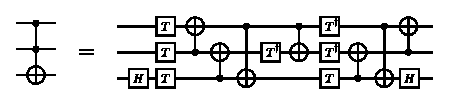
\includegraphics[scale=1.5]{images/toffoli}
 \caption{A $T$-depth 3 version of the Toffoli gate over Clifford+$T$. 
 This circuit has full depth 9. 
 Figure reproduced from Figure 13 of \cite{MITM}.}
 \label{fig:toffoli-tdepth-3}
\end{figure}


The number of qubits required was explained previously, but let's total them up. 
Suppose that our memory addresses are $n$ bits. 
Then:
\begin{equation}
 \begin{tabular}{c|c}
  Register & Number  of qubits \\ \hline
  $a$ & $n$ \\
  $\tau$ & $2^n$ \\
  $m$ & $2^n$ \\
  Output & 1 \\ \hline
  Total $N_q$ & $2^{n+1} + n + 1$
 \end{tabular}
\end{equation} 

Next, let's take a closer look at the gate counts. 
In the fanout portion, we see there are $2^n - 2$ Toffolis, and $2^n$ CNOTs. 
In the case where the auxiliary register is being re-used, the fanout portion must be run twice \todo{(depending on how the library handles aux registers, we may not actually need this)}, yielding $2^{n+1} - 4$ Toffolis and $2^{n+1}$ CNOTs. 
As for the query portion, we see there are $2^n$ sequential Toffolis.

Let us begin by computing the $T$-count $N_T$. 
Each Toffoli has 7 $T$-gates, so we have
\begin{eqnarray}
 \nonumber N_T &=& 2 \cdot N_T(\hbox{fanout}) + N_T(\hbox{query}) \\
 \nonumber    &=& 2 \cdot 7 \cdot (2^n - 2) + 7 \cdot 2^n \\
     &=& 21 \cdot 2^n - 28
\end{eqnarray}

Next, the $T$-depth of all the Toffolis. 
Since none of the Toffolis are parallelized, it is just the sum of the $T$-depth of the individual gates:
\begin{eqnarray}
 \nonumber D_T &=& 2 \cdot D_T(\hbox{fanout}) + D_T(\hbox{query}) \\
 \nonumber    &=& 2 \cdot 3 \cdot (2^n - 2) + 3 \cdot 2^n \\
     &=& 9 \cdot 2^n - 12
\end{eqnarray}

The number of non-$CNOT$ Cliffords is also straightforward; only the Toffolis have any such gates: 2 Hadamards per Toffoli. 
Thus,
\begin{eqnarray}
 \nonumber N_{HS} &=& 2 \cdot N_{HS}(\hbox{fanout}) + N_{HS}(\hbox{query}) \\
 \nonumber    &=& 2 \cdot 2 \cdot (2^n - 2) + 2 \cdot 2^n \\
     &=& 6 \cdot 2^n - 8
\end{eqnarray}

For $N_{CX}$, we have
\begin{eqnarray}
 \nonumber N_{CX} &=& 2 \cdot N_{CX}(\hbox{fanout}) + N_{CX}(\hbox{query}) \\
 \nonumber    &=& 2 \cdot \left(7 \cdot (2^n - 2) + 2^n \right)  + 7 \cdot 2^n \\
     &=& 23 \cdot 2^n - 28
\end{eqnarray}

Finally, let's compute the depth. 
Note that in the fanout portion, the CNOTs can be run in only $n + 1$ layers of depth because many of the cascades can be parallelized. 
The depth of the Toffolis, however, is fixed at 9, so we obtain:
\begin{eqnarray}
 \nonumber D &=& 2 \cdot D (\hbox{fanout}) + D (\hbox{query}) \\
 \nonumber    &=& 2 \cdot \left(9 \cdot (2^n - 2) +n + 1 \right) + 9 \cdot 2^n \\
     &=& 27 \cdot 2^n + 2n -34
\end{eqnarray}

The final (unoptimized) resource counts for a one-bit bucket brigade qRAM are:
\begin{eqnarray}
 N_q &=& 2^{n+1} + n + 1 \\ \nonumber
 D   &=& 27 \cdot 2^n + 2n -34 \\ \nonumber
 D_T &=& 9 \cdot 2^n - 12 \\ \nonumber
 N_T &=& 21 \cdot 2^n - 28 \\ \nonumber
 N_{CX} &=& 23 \cdot 2^n - 28 \\ \nonumber
 N_{HS} &=& 6 \cdot 2^n - 8
\end{eqnarray}
 
 
 \todo{VERIFY and cross-check with \texttt{ResourcesEstimator} and our library code.}
 
\paragraph{Multi-bit output}

Let us now perform the same analysis for the situation where the memory cells may store multiple bits.
We'll suppose that addresses are still $n$ bits, but store $k$ bits each. 
Consider the differences between the top right panel of \autoref{fig:bb-combined}, and \autoref{fig:bb-multioutput} (i.e. a 2-bit address, so 4 memory cells). 
The address fanout portion is \emph{exactly the same}; what differs is the query itself, as now we need to couple with each of the memory cells to copy the information to the output.
The number of qubits of course increases:
\begin{equation}
 \begin{tabular}{c|c}
  Register & Number  of qubits \\ \hline
  $a$ & $n$ \\
  $\tau$ & $2^n$ \\
  $m$ & $k \cdot 2^n$ \\
  Output & $k$ \\ \hline
  Total $N_q$ & $(k + 1) 2^n + n + k$
 \end{tabular}
\end{equation} 
Then each of the $2^n$ Toffolis of the query portion is replaced with $k$ Toffolis, one per output bit.
Note, however, that many of these Toffolis can in fact be done in parallel. 
We will not consider that when estimating resources here by hand, but note that once we implement the circuits in Q\# and use the Toffoli simulator, the circuit depth will likely decrease significantly.
Calculating by hand, the resources for the multi-output bit case are as follows:
\begin{eqnarray}
 N_q &=& (k + 1) 2^n + n + k \\ \nonumber
 D   &=& (18 + 9k)2^n + 2n - 34 \\ \nonumber
 D_T &=& (6+3k)2^n - 12 \\ \nonumber
 N_T &=& (14 + 7k)2^n - 28 \\ \nonumber
 N_{CX} &=& (16+7k)2^n - 28  \\ \nonumber
 N_{HS} &=& (4+2k)2^n - 8
\end{eqnarray}

\todo{Verify and cross-check with \texttt{ResourcesEstimator}}


\subsection{Phase query circuit model}

In some situations, most notably in Grover's algorithm\footnote{A \href{https://github.com/qsharp-community/qram/tree/master/samples/Grover}{sample implementation of Grover's algorithm} is included in the Q\# qRAM library}, one is concerned with retrieving the memory contents not in bit form, but as a phase. 
Explicitly, 
\begin{equation}
 \ket{i} \rightarrow (-1)^{m_i} \ket{i}
\end{equation}

Such a query can be done using slight modifications from the bucket brigade model.
In particular, all that must be done is to start with the target in the state $\ket{1}$, and replace the Toffolis in the query with CCZs.
An example is shown in \autoref{fig:bb-phase-query} for a 2-bit address. 
This circuit can be parallelized using the same techniques as shown in \autoref{fig:bb_2address_ccz_full}.
In fact, the only difference is that the target qubit starts in $\ket{1}$, and the Hadamards are removed.

\begin{figure}[ht!]
 \centering
  \captionsetup{width=.89\linewidth}
 \includegraphics[scale=0.7]{images/bb_phase_query}
 \caption{Bucket-brigade style circuit that performs the query $\ket{i} \rightarrow (-1)^{m_i}\ket{i}$, where $m_i$ is  the contents of the memory at address $\ket{i}$.
 Note that the target qubit starts in $\ket{1}$ allow for phase kickback with the CCZ; the CCZ triggers only if all of the auxiliary, memory, and targets are in $\ket{1}$.}
 \label{fig:bb-phase-query}
\end{figure}

%%%%%%%%%%%%%%%%%%%%%%%%%%%%%%%%%%%%%%%%%%%%%%%%%%%%%%%%%%%%%%%%%%%%%%%%%%%%%%%%%%
%%%%%%%%%%%%%%%%%%%%%%%%%%%%%%%%%%%%%%%%%%%%%%%%%%%%%%%%%%%%%%%%%%%%%%%%%%%%%%%%%%
%%%%%%%%%%%%%%%%%%%%%%%%%%%%%%%%%%%%%%%%%%%%%%%%%%%%%%%%%%%%%%%%%%%%%%%%%%%%%%%%%%
%%%%%%%%%%%%%%%%%%%%%%%%%%%%%%%%%%%%%%%%%%%%%%%%%%%%%%%%%%%%%%%%%%%%%%%%%%%%%%%%%%
%%%%%%%%%%%%%%%%%%%%%%%%%%%%%%%%%%%%%%%%%%%%%%%%%%%%%%%%%%%%%%%%%%%%%%%%%%%%%%%%%%

\section{Quantum ROM}
\label{sec:qrom}

The distinguishing feature of RAM is that elements in the memory can be read or written arbitrarily, in any order. 
It is assumed that its contents will change over time. 
However, there are other situations where perhaps one does not intend to change the memory contents (or at least, not very frequently). 
While there are many types of ROMs with varying degrees of reusability, conceptually we will consider ROM (and qROM) as a look up table. 
We have some known, relatively fixed set of values at specified addresses, and we want to be able to query them in superposition.

\subsection{A simple qROM}
\label{subsec:naive-qrom}

An advantage of the bucket-brigade type qRAMs discussed earlier is that actual qubits store the memory contents in a completely separate register. This can be treated as a black box, in that the contents of the memory have no effect on the structure or resource requirements of the query circuit. A disadvantage in practice, of course, is that those memory qubits have to be initialized and maintain coherence throughout the entire quantum algorithm.

Having knowledge about the memory contents allows for a different approach. Let's suppose we have a quantum memory with a 4-bit address that stores a single bit in each memory cell (the arguments here extend naturally to the case of multi-bit data). Now, suppose that we know which of those memory cells contain a 1 (the rest of course contain a 0). A straightforward way of designing a qROM is to construct a circuit that takes an address register and flips a target bit from $\ket{0}$ to $\ket{1}$ if the input address is known to have a 1.

As a concrete example, consider the circuit in \autoref{fig:basic-qrom}. This is a qROM for a 4-bit address. Five of the memory cells contain a 1: 0001, 0011, 0101, 1011, 1101. To perform a query, for each address that contains a 1 we add a mixed-polarity multi-controlled Toffoli (MPMCT) operation that will ``catch'' the associated address. For example, if the address 0001 is queried, the first MPMCT in the circuit (3 white controls, 1 black) will be triggered and flip the output bit, while none of the subsequent operations will occur. Similarly, if we query at address 1101, the final MPMCT of the circuit will go off, but none of the prior ones will, so the target bit flipped exactly once. For any addresses that contain a 0, none of the MPMCTs will run and the target bit remains in its initial state. As all of these operations are unitary, we can use this qROM to query in superposition. 



\begin{figure}
 \centering
 \captionsetup{width=0.89\linewidth}
 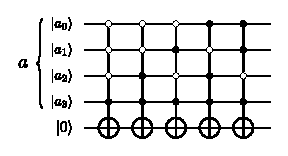
\includegraphics[scale=1.6]{images/basic-qrom}
 \caption{A basic qROM with 4-bit addresses and a single data bit stored at each. This qROM is for a memory in which exactly 5 of the 16 addresses contain a 1: 0001, 0011, 0101, 1011, 1101. Each of these address corresponds to a mixed-polarity multi-controlled Toffoli (MPMCT) gate that will flip the target bit when the associated address is fed in.}
 \label{fig:basic-qrom}
\end{figure}

\subsubsection{Resource estimation with \textsc{Exorcism-4}}

The ``naive'' way to estimate resources for a circuit of the type in \autoref{fig:basic-qrom} is to first compute the resources required for a single $n$-bit MPMCT, and then multiply by the number of 1s in the memory. While this will give us an estimate of the resources, it will not be the best one available - in fact, it represents the worst case!

Circuits like that in \autoref{fig:basic-qrom} are a special type of circuit called a \emph{reversible} circuit. While all unitary operations are reversible in the sense that they can be run ``backwards'', reversible circuit here refers specifically to circuits that represent Boolean functions, i.e. can be expressed only in terms of CNOTs, Toffolis, and $n$-qubit controlled gates. For circuits of this type, we can dive into the extensive literature of classical optimization techniques for Boolean functions. 

One such tool is called \textsc{Exorcism-4} \cite{Mishchenko2001}. \textsc{Exorcism-4} acts on Boolean functions represented in ESOP (exclusive-OR sum of product) form.
While the name is descriptive, it is always helpful to see an example.
Consider again the circuit in \autoref{fig:basic-qrom}. 
Each MPMCT can be expressed as a product term of the variables that multiplies to 1 for the correct input address.
Then, all of these product terms are summed together with the exclusive-OR (XOR) operation\footnote{XOR, denoted by $\oplus$, is essentially addition modulo 2: $0 \oplus 0 = 1 \oplus 1 = 0$, and $0 \oplus 1 = 1 \oplus 0 = 1$.}.
Explicitly,
\begin{equation}
 f(a_0, a_1, a_2, a_3) = \bar{a}_0 \bar{a}_1 \bar{a}_2 a_3 \oplus \bar{a}_0 \bar{a}_1 a_2 a_3 \oplus \bar{a}_0 a_1 \bar{a}_2 a_3 \oplus a_0 \bar{a}_1 a_2 a_3 \oplus a_0 a_1 \bar{a}_2 a_3,
\end{equation}
where $\bar{a}$ denotes NOT($a$).
If we feed $f$ an address that contains a 1, the associated product term will evalaute to 1 while the rest are 0, and the combined XOR of all terms will be 1.
If an address storing 0 is input, then none of the product terms produce a 1 and the output is 0.

Using the implementation of \textsc{Exorcism-4} provided in \texttt{abc} \cite{abc}, we can simplify the circuit in \autoref{fig:basic-qrom} to obtain a significantly smaller circuit, depicted in \autoref{fig:basic-qrom-exorcised}. 
Rather than having five 4-controlled gates, it can be reduced to one 4-controlled gate and two Toffolis! 
It would be interesting to determine if this a typical improvement.

\begin{figure}[ht]
 \centering
 \captionsetup{width=0.89\linewidth}
 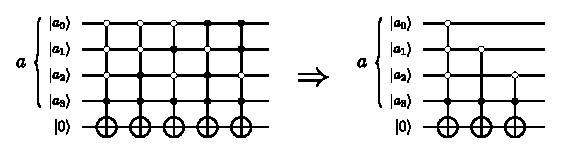
\includegraphics[scale=1.6]{images/basic-qrom-exorcised}
 \caption{Basic qROMs can be greatly simplified using Boolean circuit optimization techniques. On the right is shown an optimized version of the circuit on the left, obtained using EXORCISM-4. The resource counts are significantly reduced. Understanding what savings are available on average is an interesting research topic.}
 \label{fig:basic-qrom-exorcised}
\end{figure}

To test this, we generated random memories and computed resources before and after optimization with \textsc{Exorcism-4}. 
For each number of address bits $n = 5, \ldots 14$, we generated 1000 random qROMs where $2^{n-1}$ memory cells contain a 1.
As $T$-count and $T$-depth are typically the metrics of interest, we present them in \autoref{fig:qrom-exorcism-tcount} and \autoref{fig:qrom-exorcism-tdepth}. 

\begin{figure}[ht]
 \centering
 \captionsetup{width=0.89\linewidth}
 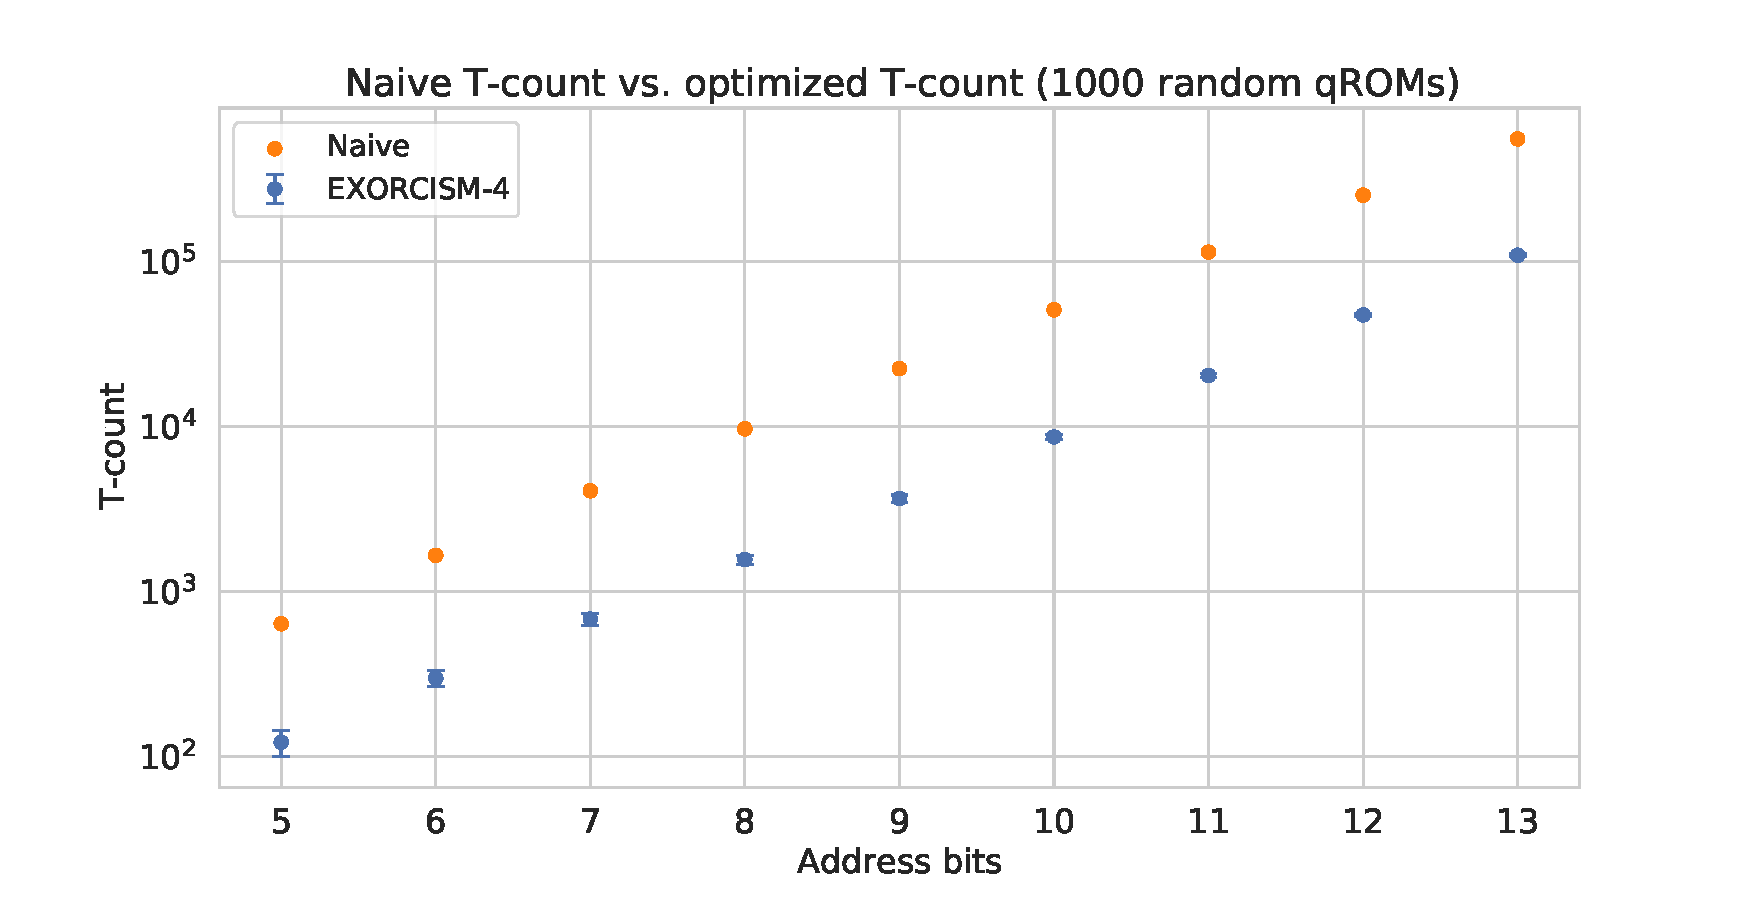
\includegraphics[scale=0.55]{images/exorcism-t-count}
 \caption{$T$-counts averaged over 1000 random, half-full qROMs computed from naive resource estimation (as per \cite{DiMatteo2020}) and optimization with \textsc{Exorcism-4}. Optimization yields a little shy of an order of magnitude reduction in $T$-count.}
 \label{fig:qrom-exorcism-tcount}
\end{figure}

\begin{figure}[ht]
 \centering
 \captionsetup{width=0.89\linewidth}
 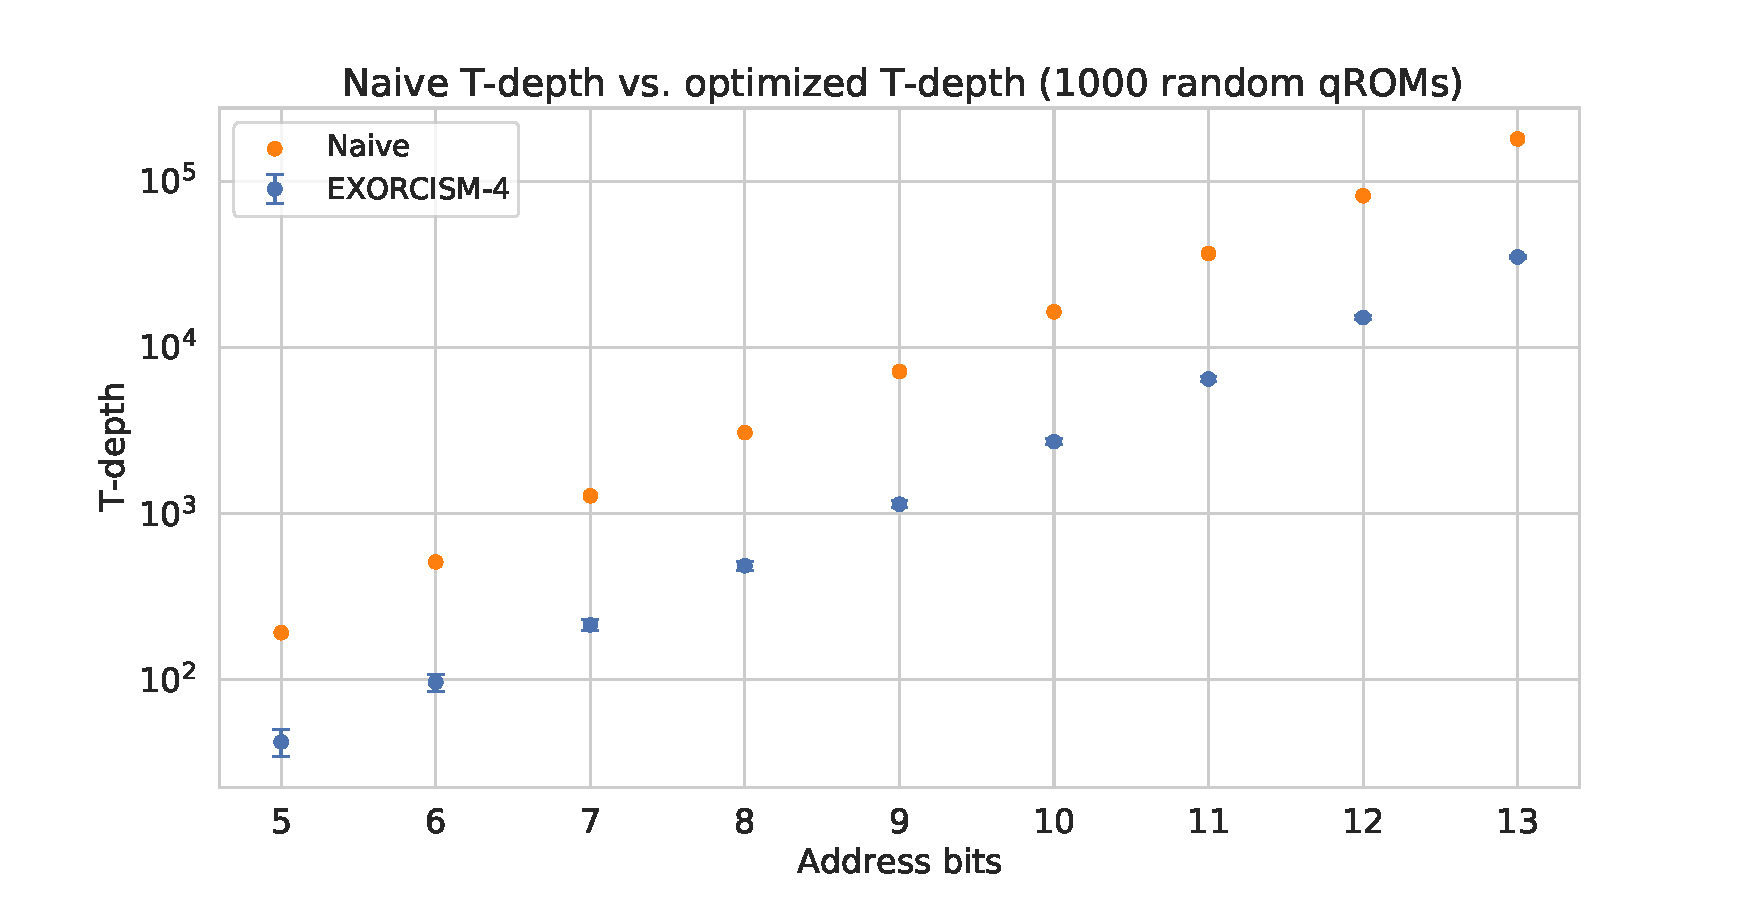
\includegraphics[scale=0.55]{images/exorcism-t-depth}
 \caption{$T$-depth of 1000 random qROMs computed from naive resource estimation (as per \cite{DiMatteo2020}) and optimization with \textsc{Exorcism-4}. As with $T$-count, optimization yielded a less than an order of magnitude reduction in $T$-depth.}
 \label{fig:qrom-exorcism-tdepth}
\end{figure}

While we see a little less than an order of magnitude reduction in both $T$-count and depth, the scaling with address size doesn't undergo any fundamental changes.
\todo{Try exorcism with the case of fixed $n$ and varying memory fullness to see how savings depend on sparsity. Maybe something neat there.}
To obtain further improvement, we have to look to different circuit constructions.

%%%%%%%%%%%%%%%%%%%%%%%%%%%%%%%%%%%%%%%%%%%%%%%%%%%%%%%%%%%%%

\subsection{\textsc{SelectSwap} qROM}

The qROM in \autoref{fig:basic-qrom} represents just one extreme of a spectrum of space-time tradeoffs that can be made. 
One not-so-efficient way of making that tradeoff is to make multiple copies of the address register, perform all the MPMCTs in parallel, and then apply a parity operation of those results to get the output bit. 
While this works, and would work quickly, the qubit overhead is \emph{astronomical} and so this isn't really something we would want to do in practice \cite{DiMatteo2020}. 
Instead it pays to look for something in between the two extremes - can we add \emph{some} extra qubits to reduce the time without going full parallel?

Some ``hybrid'' circuits to that effect were explored in \cite{DiMatteo2018, DiMatteo2020}, though around the same time as \cite{DiMatteo2018}, a better approach was presented in \cite{Vadym2018}. 
These are called the \textsc{SelectSwap} circuits, after their two-part structure: a \textsc{Select} operation, and a \textsc{Swap} operation.

\begin{figure}[ht]
 \centering
 \captionsetup{width=0.89\linewidth}
 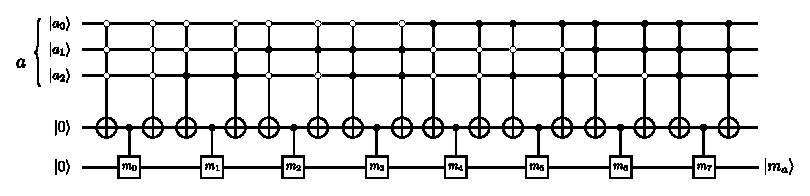
\includegraphics[scale=1.2]{images/select-swap-only-select}
 \caption{A \textsc{Select} operation being used as a qROM for a 3-bit address space. The controlled-$m$ blocks indicate application of Pauli $X$ gates according to the bit strings in memory $m_i$.}
 \label{fig:select-swap-only-select}
\end{figure}

The \textsc{Select} operation is what's known as a multiplexing operation.
Suppose we have a set of $2^n$ unitaries $\{U_i\}$ that we would like to apply conditioned on different basis states.
For example, if a set of control qubits is in the state $\ket{00\cdots0}$, we want to apply $U_0$ to a set of target qubits.
If the control qubits are in state $\ket{00\cdots1}$, we apply $U_1$, and so on.
\textsc{Select} is expressed mathematically as 
\begin{equation}
 \textsc{Select} = \sum_{i=0}^{2^n - 1} \ket{i}\bra{i} \otimes U_i.
\end{equation}
Recall that a qROM is a circuit designed to output specific memory contents based on the address that is fed in.
We can use \textsc{Select} to perform this task, and an example circuit is presented in \autoref{fig:select-swap-only-select}.
The first register (the $\ket{i} \bra{i}$ part of the equation) represents a controlled operation from a register of address bits.
Then, the $U_i$ is an operation that writes the appropriate memory contents at cell $i$ to a target register. 
Note that a key difference between \textsc{Select} and the naive qROMs of \autoref{subsec:naive-qrom} is that the \textsc{Select} operation cycles through \emph{all} possible addresses, whereas the naive qROM only includes gates for addresses that contain a 1.
Running through the full address space leads to some interesting optimization methods that rely on this \todo{cite relevant paper}.
\todo{Say something about uniformly controlled rotations?}

The \textsc{Swap} operation comes into play when we begin to parallelize.
Rather than controlling on all $n$ address bits, what if we controlled on only some of them, and used those results to perform further processing?
This would lead to less complex operations, but potentially additional qubit overhead.
In what follows we will discuss a somewhat simplified version of the original circuits in \cite{Vadym2018}.

\begin{figure}[ht!]
\centering
 \captionsetup{width=0.89\linewidth}
\begin{subfigure}{0.6\textwidth}
 \centering
 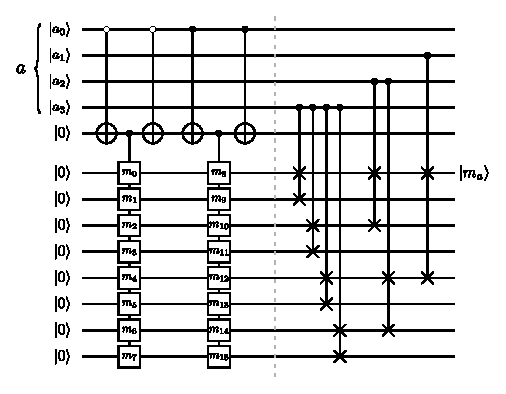
\includegraphics[scale=1.3]{images/select-swap-lambda-1}
 \caption{Tradeoff parameter 1.}
 \label{fig:select-swap-1}
 \end{subfigure} \\ \vspace{0.5cm}
\begin{subfigure}[ht!]{0.8\textwidth}
 \centering
 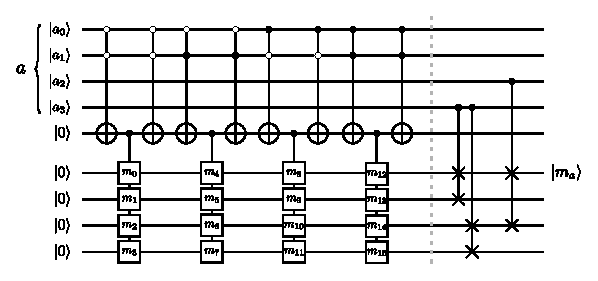
\includegraphics[scale=1.3]{images/select-swap-lambda-2}
 \caption{Tradeoff parameter 2.}
 \label{fig:select-swap-2}
 \end{subfigure} \\ \vspace{0.5cm}
\begin{subfigure}[ht!]{\textwidth}
 \centering
 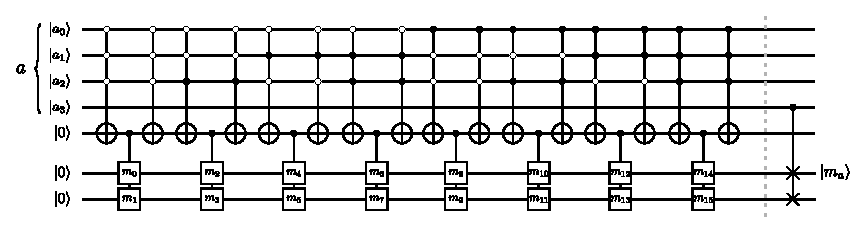
\includegraphics[scale=1.3]{images/select-swap-lambda-3}
 \caption{Tradeoff parameter 3.}
 \label{fig:select-swap-3}
 \end{subfigure}
 \caption{Highlighting the space time tradeoffs available from the \textsc{SelectSwap} qROM. Boxes labeled by $m_i$ indicate the memory contents stored at address $i$. While only a single qubit is shown, these may be multi-bit values. The circuits consist of a \textsc{Select}  operation to identify the correct memory cells, followed by a \textsc{Swap}  network to move the desired contents to a target register (not shown: the memory contents would have to be copied to a final output register with a cascade of CNOTs.) A tradeoff parameter controls the relative size of the two operations, and consequently the depth and width of the circuit.}
 \label{fig:select-swap}
\end{figure} 

\todo{I'm not really happy with this explanation - suggestions welcome. A lot of my conceptual understanding comes from looking at the circuit diagrams, and I'm having a hard time expressing it verbally.}

These are best explained visually, and a number of examples are shown in \autoref{fig:select-swap}.
In \textsc{SelectSwap} circuits, the address space is partitioned, and multiple copies of an output register are made depending on how many qubits are split off in the partitioning.
Rather than performing the full-size MPMCTs, one with only a subset of the address bits is performed, and it writes to the output register all the memory contents where that subset of addresses match.
Then, the remaining address bits are used to perform a sequence of controlled Swap operations.
This effectively moves the desired memory contents to an output register.

The tradeoff lies in how the address space is partitioned.
As in \autoref{fig:select-swap}, for a 4-bit space (16 memory cells) we can partition three ways.
In \autoref{fig:select-swap-1}, the first address bit is separated from the rest, and 8 copies of the output register are made (because separating the first bit divides the space in 2).
The select operation then has two portions, one which writes the first 8 contents where the first address bit is 0, and another that writes the 8 contents where the first address bit is 1.
The remaining three address bits are then used to swap these contents up to a specified location to be read out.
Similarly, we can control on the first two address bits, and partition the space into 4 sets of 4, as in \autoref{fig:select-swap-2}. 
Here the MPMCTs in \textsc{Select} get larger, the number of qubits is less than that of \autoref{fig:select-swap-1} and the swap network is smaller.
Finally in \autoref{fig:select-swap-3} we control on the first 3 address bits. 
Now only one extra copy of the output must be made and a single controlled-swap performed, but the MPMCTs have become even larger, approaching those of a standalone \textsc{Select}.

\subsubsection{Resource estimation}

A nice resource analysis of \textsc{SelectSwap} is provided in the original work \cite{Vadym2018}.
A key feature of these circuits is that one can solve for an \emph{optimum} tradeoff parameter.
Namely, how many copies of the output register should we make to get the best qubit-time tradeoff?
\todo{More details. Discuss $\lambda = O(\sqrt{N})$, and $T$-count / $T$-depth results.}

\subsection{Problem-specific qROMs}

Talk about the qROM in \cite{Babbush2018}
%%%%%%%%%%%%%%%%%%%%%%%%%%%%%%%%%%%%%%%%%%%%%%%%%%%%%%%%%%%%%%%%%%%%%%%%%%%%%%%%%%
%%%%%%%%%%%%%%%%%%%%%%%%%%%%%%%%%%%%%%%%%%%%%%%%%%%%%%%%%%%%%%%%%%%%%%%%%%%%%%%%%%
%%%%%%%%%%%%%%%%%%%%%%%%%%%%%%%%%%%%%%%%%%%%%%%%%%%%%%%%%%%%%%%%%%%%%%%%%%%%%%%%%%
%%%%%%%%%%%%%%%%%%%%%%%%%%%%%%%%%%%%%%%%%%%%%%%%%%%%%%%%%%%%%%%%%%%%%%%%%%%%%%%%%%
%%%%%%%%%%%%%%%%%%%%%%%%%%%%%%%%%%%%%%%%%%%%%%%%%%%%%%%%%%%%%%%%%%%%%%%%%%%%%%%%%%

\section{Hardware proposals for qRAM}
\label{sec:hardware}



%%%%%%%%%%%%%%%%%%%%%%%%%%%%%%%%%%%%%%%%%%%%%%%%%%%%%%%%%%%%%%%%%%%%%%%%%%%%%%%%%%
%%%%%%%%%%%%%%%%%%%%%%%%%%%%%%%%%%%%%%%%%%%%%%%%%%%%%%%%%%%%%%%%%%%%%%%%%%%%%%%%%%
%%%%%%%%%%%%%%%%%%%%%%%%%%%%%%%%%%%%%%%%%%%%%%%%%%%%%%%%%%%%%%%%%%%%%%%%%%%%%%%%%%
%%%%%%%%%%%%%%%%%%%%%%%%%%%%%%%%%%%%%%%%%%%%%%%%%%%%%%%%%%%%%%%%%%%%%%%%%%%%%%%%%%
%%%%%%%%%%%%%%%%%%%%%%%%%%%%%%%%%%%%%%%%%%%%%%%%%%%%%%%%%%%%%%%%%%%%%%%%%%%%%%%%%%

\section{Outlook}
\label{sec:outlook}

%%%%%%%%%%%%%%%%%%%%%%%%%%%%%%%%%%%%%%%%%%%%%%%%%%%%%%%%%%%%%%%%%%%%%%%%%%%%%%%%%%
%%%%%%%%%%%%%%%%%%%%%%%%%%%%%%%%%%%%%%%%%%%%%%%%%%%%%%%%%%%%%%%%%%%%%%%%%%%%%%%%%%
%%%%%%%%%%%%%%%%%%%%%%%%%%%%%%%%%%%%%%%%%%%%%%%%%%%%%%%%%%%%%%%%%%%%%%%%%%%%%%%%%%
%%%%%%%%%%%%%%%%%%%%%%%%%%%%%%%%%%%%%%%%%%%%%%%%%%%%%%%%%%%%%%%%%%%%%%%%%%%%%%%%%%
%%%%%%%%%%%%%%%%%%%%%%%%%%%%%%%%%%%%%%%%%%%%%%%%%%%%%%%%%%%%%%%%%%%%%%%%%%%%%%%%%%

\bibliography{primer}
\bibliographystyle{unsrt}

\appendix


\section{Improving $T$ depth of bucket-brigade qRAM with the CCZ gate}

Looking at the circuits of \autoref{fig:bb-combined}, one notes that there are many instances of sequential Toffolis. 
In \cite{DiMatteo2020}, a parallelized version of the circuit was proposed. 
In the fanout, multiple copies of the address bits were made so the Toffolis could be performed in parallel. 
The query portion was parallelized by giving each Toffoli a different target qubit, and then taking the parity of those bits using CNOT gates. 
This works fine, and has the effect of reducing the $T$-depth from $O(2^n)$ to $O(n)$. 
However, it comes at a significant cost: the number of auxiliary qubits that must be added is $O(2^n)$.

\todo{These sections are rough, and will be re-written as I make my way through \cite{Alexandru2020}.}
The authors of \cite{Alexandru2020} found a more efficient way to parallelize this by taking advantage of some circuit identities that can be applied when two neighbouring Toffolis share a control bit. 
In fact, this gives a significant advantage - the $T$-depth will go from $O(2^n)$ to $O(n)$ \emph{without} adding any auxiliary qubits!

\begin{figure}[ht]
 \centering 
 \captionsetup{width=.89\linewidth}
 \includegraphics[scale=2]{images/ccz}
 \caption{A Toffoli can be re-written as a controlled-controlled-$Z$ gate with its target qubit conjugated by Hadamards.}
 \label{fig:ccz}
\end{figure}

\begin{figure}[ht]
 \centering
  \captionsetup{width=.89\linewidth}
 \includegraphics[scale=0.8]{images/ccz-clifford-t}
 \caption{Decomposition of CCZ over Clifford+$T$ gate set. It requires 7 $T$ gates, has $T$ depth 4, and total depth 10.}
 \label{fig:ccz-clifford-t}
\end{figure}

The trick involves replacing the Toffoli gates with controlled-controlled-$Z$ (CCZ) gates, as per the identity shown in \autoref{fig:ccz}. The CCZ gate perform the operation
\begin{equation}
 CCZ \ket{b_0 b_1 b_2} = (-1)^{b_0 b_1 b_2} \ket{b_0 b_1 b_2}
\end{equation}
In other words, the phase of the state is flipped only if all three qubits are in $\ket{1}$. Note that due to this symmetry, qubits in a CCZ lose the distinction of target/control. 
The CCZ can be done with the qubits in `any order', as the only time the state is affected is when all qubits are in the same state anyways.
Thus, every Toffoli in the bucket brigade cricuits can be turned into a CCZ by simply conjugating the target by Hadamard gates. 


To see how the $T$-depth is reduced when working in terms of CCZ, we refer to the Clifford+$T$ decomposition shown in \autoref{fig:ccz-clifford-t}. 
The $T$-count of this circuit is 7 (as is the Toffoli), and its $T$ depth is 4. 
The magic happens when two adjacent CCZs share a control bit. 
An example is shown in \autoref{fig:bb-ccz-simplification}. 
Using the decomposition of \autoref{fig:ccz-clifford-t}, we can rewrite the cascades of Toffolis that occur from the address bits to the auxiliary register. 
Note that this \emph{still} has only $T$ depth 4.
Also, it has $T$-count 12 rather than 14 - the $T$ on the shared control qubit combine to form an $S$ gate, which is a Clifford. 
(Identities and notation for this circuit are shown in \autoref{fig:bb-constant-identities}.)

\begin{figure}[ht]
 \centering
  \captionsetup{width=.89\linewidth}
 \includegraphics[scale=2]{images/constant-bb-useful-identities}
 \caption{(Left) When simplifying the circuit for two CCZs sharing a control bit, we make use of the fact that a $T$ gate commutes with a CNOT when applied to the control qubit (note that this is not true for a $T$ gate applied to the target). 
 (Right) Notation for a fanout of CNOTs. This notation indicates that the same qubit is the control for multiple target qubits.}
 \label{fig:bb-constant-identities}
\end{figure}

\begin{figure}
 \centering
  \captionsetup{width=.89\linewidth}
 \includegraphics[scale=1.5]{images/ccz-simplification}
 \caption{If we apply the decomposition of \autoref{fig:ccz-clifford-t} to portions of the address fanout, we can significantly reduce the $T$ depth and circuit depth. 
 We can even reduce the $T$ count by 2, since the $T$ gates on the shared control qubit combine to form an $S$.
 Rather than having 14 $T$ gates, $T$ depth 8, and total depth 20 as one naively would expect for two CCZs in sequence, it has $T$ count 12, $T$-depth 4, and total depth $13$.}
 \label{fig:bb-ccz-simplification}
\end{figure}

The identity in \autoref{fig:bb-ccz-simplification} can be applied throughout the entire bucket brigade circuit. 
Full examples for the case of 2 and 3 address bits are shown in \autoref{fig:bb_2address_ccz_full} and \autoref{fig:bb_3address_ccz_full} respectively. 
In the query portion, recall that the initial set of Toffolis share a common target, rather than a control bit.
However once we conjugate these by Hadamards (all but the outer two cancel), we are left again with a sequence of CCZs sharing a `control' (the former target), and can make use of the same identity.

\begin{sidewaysfigure}[ht]
 \captionsetup{width=.89\linewidth}
 \includegraphics[scale=0.8]{images/bb_2address_ccz_full}
 \caption{2-address bucket brigade circuit with Toffoli cascades replaced by parallelized CCZs. 
 Note that the $T$-depth is now linear in the number of address bits ($4n$) rather than exponential as was assumed in the previous section without any optimization.
 When the query register is parallelized, there are 4 adjacent CCZs; each pair picks up an $S$ on the control bit.}
 \label{fig:bb_2address_ccz_full}
\end{sidewaysfigure}

\begin{sidewaysfigure}[ht]
 \captionsetup{width=.89\linewidth}
 \includegraphics[scale=0.5]{images/bb_3address_ccz_full}
 \caption{3-address bucket brigade circuit with Toffoli cascades as CCZs. 
 This figure should eventually be removed because it's enormous, but leaving here for now as a reference.
 Note that the $S^4$ on the target register is actually $\mathds{1}$; it's been left here for clarity.}
 \label{fig:bb_3address_ccz_full}
\end{sidewaysfigure}

In these figures, the savings in depth becomes apparent.
While the $T$-count is reduced only slightly, the $T$s have been nicely parallelized.
The query portion in particular has now only $T$ depth 4.
The fanout portion has $T$-depth $4(n-1)$: $n - 1$ of the address bits contain adjacent Toffolis, and each has depth $4$.
Taking into account the reverse of the fanout, the total $T$-depth is $8n - 4$, a significant reduction over the $9 \cdot 2^n - 12$ that was naively computed in the previous section.
In the case where the memory cells store multiple data bits, the query portion is repeatedly identically for each target bit with the same auxiliary register, but coupling to the associated memory cell. 
For $k$-bit output, the $T$-depth is thus $8n - 8 + 4k$.

\todo{Add discussion of circuit depth and complexity of `quantum fanout'.}

\end{document}
